
\chapter{$\pi$ est un nombre}\label{chap_pinombre}

\section{Introduction}

	\initial{A}{u} collège, de nombreux professeurs de mathématiques parachutent le nombre $\pi$ au milieu d'une formule magique à apprendre par c\oe{}ur\,:
	\begin{quote}
		Le périmètre d'un cercle\footnote{On rappelle que le diamètre mesure le double du rayon. Le rayon d'un cercle est la distance qui sépare le centre du cercle à sa circonférence. Le périmètre, étymologiquement, signifie la mesure du contour.} de diamètre $D$ mesure $P=\pi D$.

		Le périmètre d'un cercle de rayon $R$ mesure $P=2\pi R$.
	\end{quote}

	Et on donne une approximation numérique de $\pi$, souvent environ 3,14. Sans aucune autre forme de procès. S'ensuit la fameuse séance d'exercices, qui consiste à répéter bêtement le calcul de périmètres de cercles dont on donne les dimensions.

	D'où sort le nombre $\pi$ dans tout ça\,? Il est vraisemblable que de nombreux professeurs de mathématiques l'ignorent, ou l'ont oublié, dans la nécessité urgente de faire bouffer des compétences abrutissantes à leurs pauvres élèves, avant de s'abrutir eux-mêmes.

	Le but de ce premier chapitre est de prendre le chemin à rebours du vomi académique prodigué à nos jeunes têtes au sein de l'Éducation Nationale. Dans notre approche, nous allons considérer que le nombre $\pi$ provient d'un théorème qui n'a rien d'évident et que nous allons démontrer\,:
	\begin{thm}
		Si l'on considère n'importe quel cercle, le rapport entre son périmètre et son diamètre vaut le même nombre. On appelle $\pi$ ce nombre.

		Autrement dit, si l'on considère deux cercles quelconques de diamètres $D$ et $D'$, et de périmètres $P$ et $P'$, alors il existe un nombre réel $\pi$ tel que
		\begin{equation}
			\pi=\frac{P}{D}=\frac{P'}{D'}. \nonumber
		\end{equation}
	\end{thm}
		
	Cette idée de rapport de distance qui se conserve évoque la proportion d'une figure. Affirmer ce théorème revient en quelque sorte à dire que tous les cercles ont la même forme, quelle que soit leur taille.

	Si l'existence satisfait la plupart des mathématiciens, nous voudrions quand même calculer ce fichu nombre $\pi$. Nous n'allons pas donner la méthode la plus efficace au sens moderne\footnote{C'est-à-dire qui nécessite un nombre de calculs le plus faible possible.}, car elle nécessiterait d'utiliser des méthodes qui ne nous sont pas encore accessible. En revanche, la méthode d'Archimède est tout-à-fait accessible, car en plus de quelques notions élémentaires de géométrie euclidienne, elle ne nécessite que d'utiliser le théorème de Pythagore.

	L'approche de cette section est semi-intuitive, au sens où nous ne reconstruisons pas axiomatiquement toute la théorie géométrique, nous admettons celle qui a été prodiguée pendant \guil{maths-champignons}. Nous admettons donc les théorèmes de Pythagore et de Thalès, qui nous seront utiles pour calculer une valeur approchée du nombre $\pi$, ainsi que pour démontrer qu'il s'agit bien d'un nombre. 

\section{Longueur d'une courbe}
	Intuitivement, une courbe, ou un arc, est une ligne plus ou moins sinueuse (comme le cercle\,!). On pourrait se dire que si l'on tend cette ligne sans l'allonger ni la rétrécir, il suffirait de la mesurer avec une règle graduée pour en obtenir la longueur. Une telle opération n'est pas simple à réaliser mathématiquement, il s'agirait de déformer une courbe sans modifier sa longueur\,: on appelle cela une déformation isométrique\footnote{iso=même, métrique=mesure.}. Mais cela nous fait tourner en rond, puisque nous n'avons toujours pas défini la mesure d'un arc. L'intuition est donc ici insuffisante pour définir correctement les longueurs.

	L'objet de cette section n'étant pas d'étudier avec précision les arcs paramétrés, nous en donnerons ici un exposé semi-intuitif qui sera approfondi lors de prochaines séances.

	Considérons une courbe du plan comme dans la figure \ref{fig_courbe}. On voudrait mesurer sa longueur. Pour l'instant, nous ne savons pas mesurer autre chose que des lignes droites, or ici nous avons affaire à une ligne courbe. Pour résoudre le problème, nous allons approcher cette courbe par une ligne brisée. La première approche sera grossière, la seconde un peu plus fine, et ainsi de suite à l'infini. Et alors, nous définirons la longueur de la courbe comme la longueur de la ligne infiniment brisée qui se rapproche infiniment de la courbe (voir figure \ref{fig_ligne_brisee}).

	\begin{figure}
		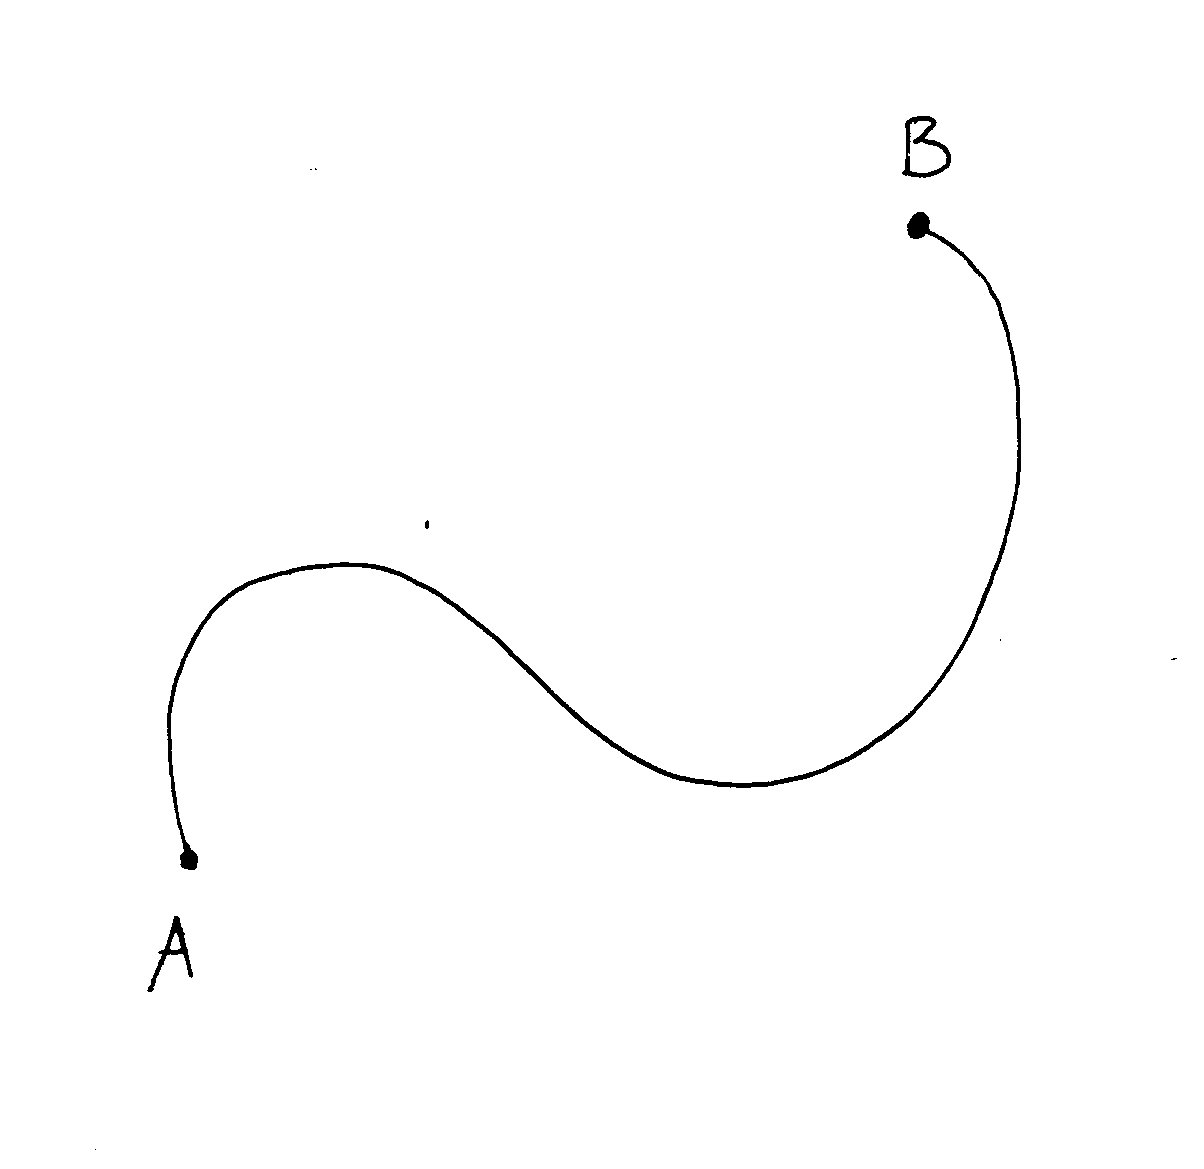
\includegraphics[width=0.4\textwidth]{image/pi_nombre/courbe1.jpg}
		\caption{Exemple de courbe comprise entre deux points $A$ et $B$.}	\label{fig_courbe}
	\end{figure} 

	Dans la première approximation de la figure \ref{fig_ligne_brisee}, une valeur approchée de la longueur $\mathscr{L}$ de la ligne comprise entre $A$ et $B$ est $AC+CD+DE+EB$. Plus la subdivision est fine, plus la ligne brisée est proche de la courbe\,: avec la ligne brisée verte, une valeur approchée de la longueur $\mathscr{L}$ serait ensuite $AF+FG+GC+CH+HI+ID+DJ+JK+KE+EL+LM+MB$. En bas, on a représenté un zoom pour montrer qu'il est toujours possible d'affiner la subdivision\,: on pourrait ajouter des points entre la subdivision de la ligne rouge.

	\begin{figure}
		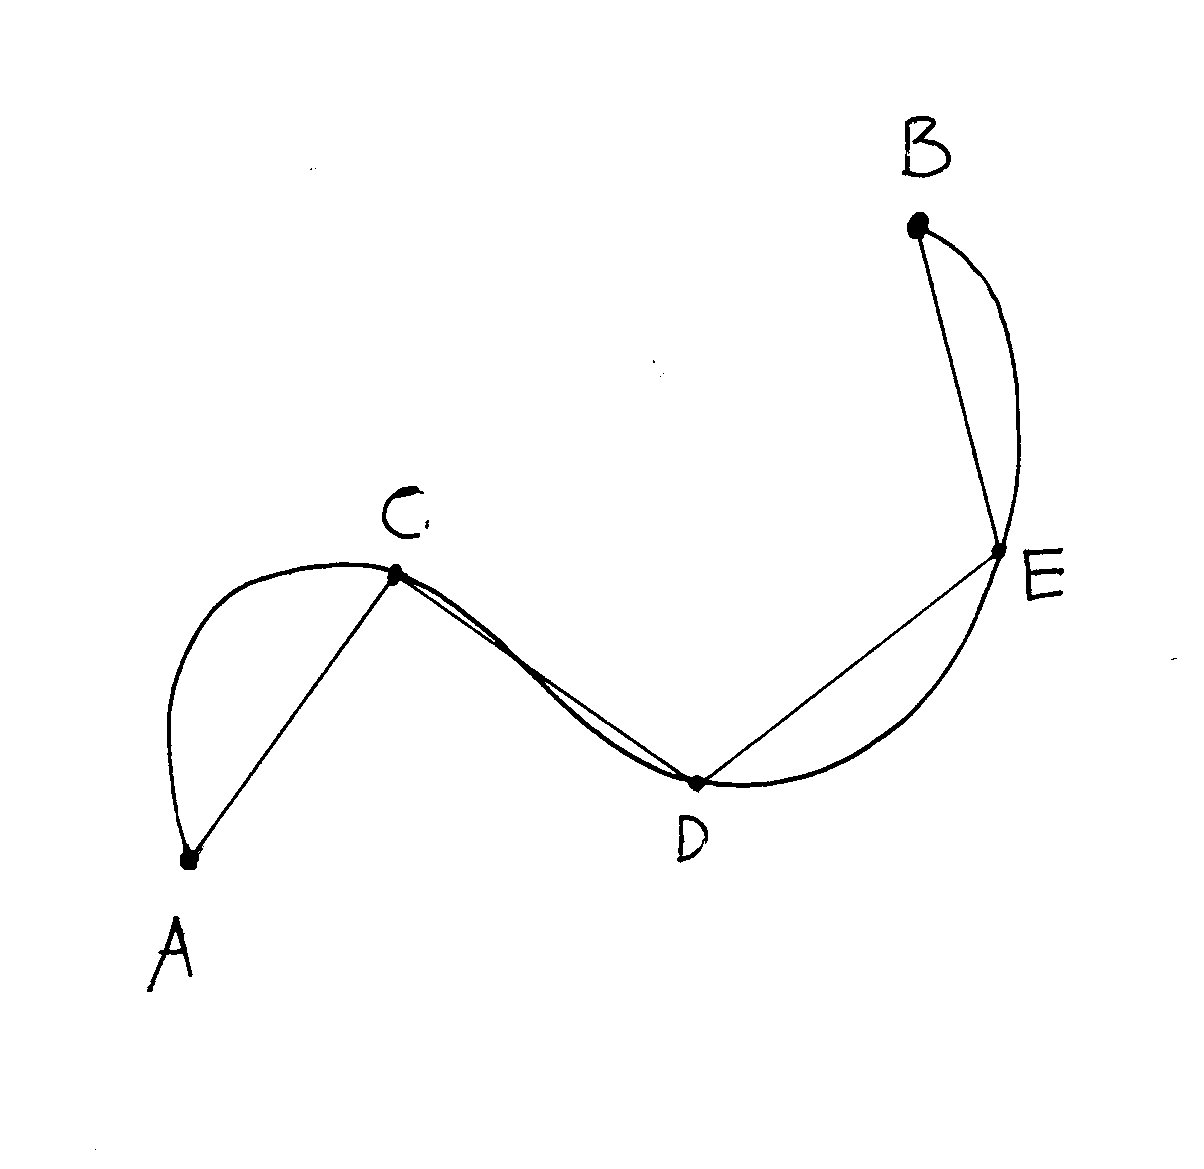
\includegraphics[width=0.45\textwidth]{image/pi_nombre/courbe2.jpg}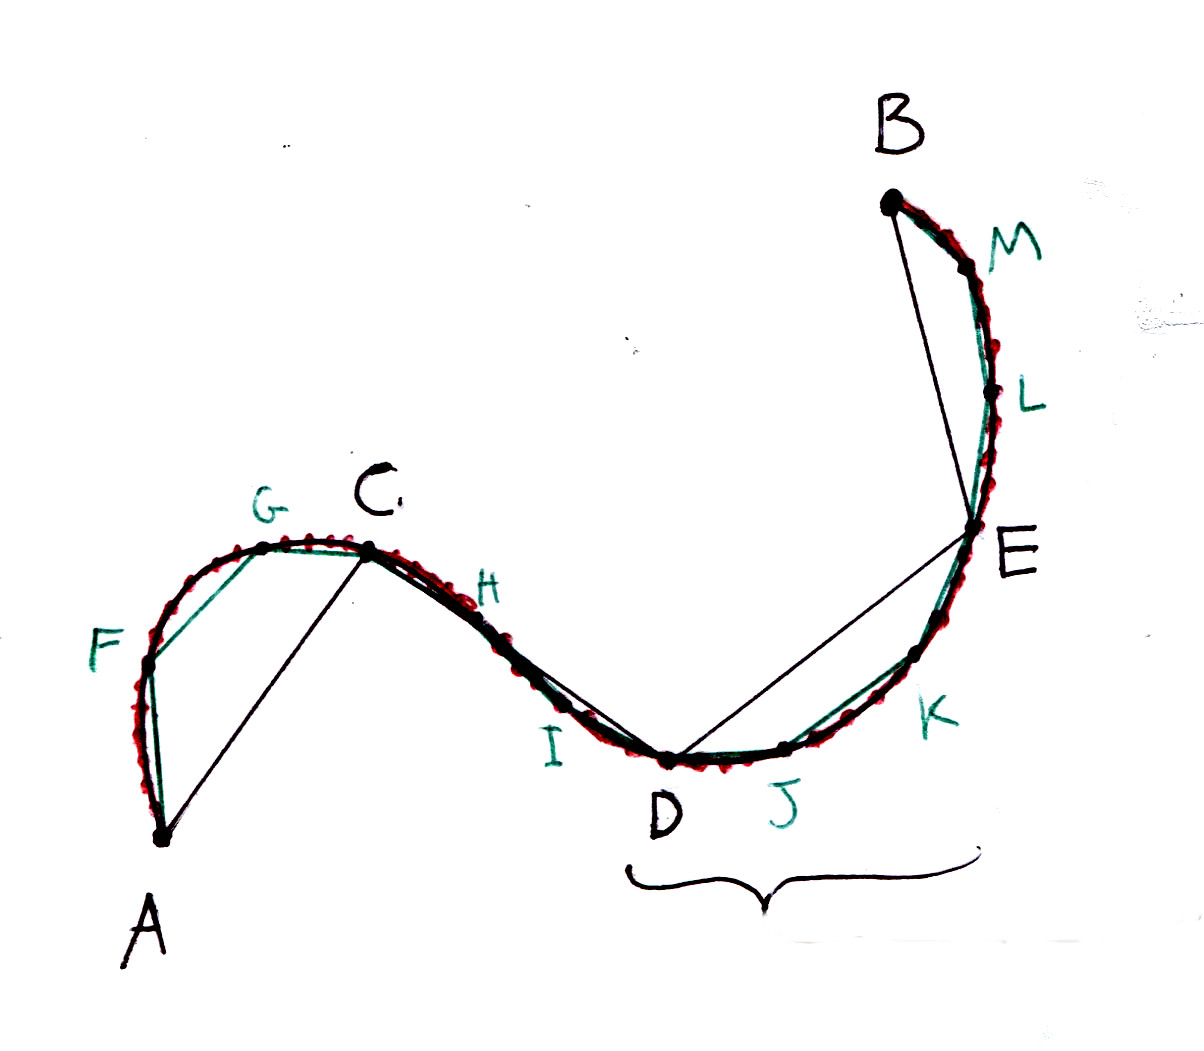
\includegraphics[width=0.45\textwidth]{image/pi_nombre/courbe3.jpg}

		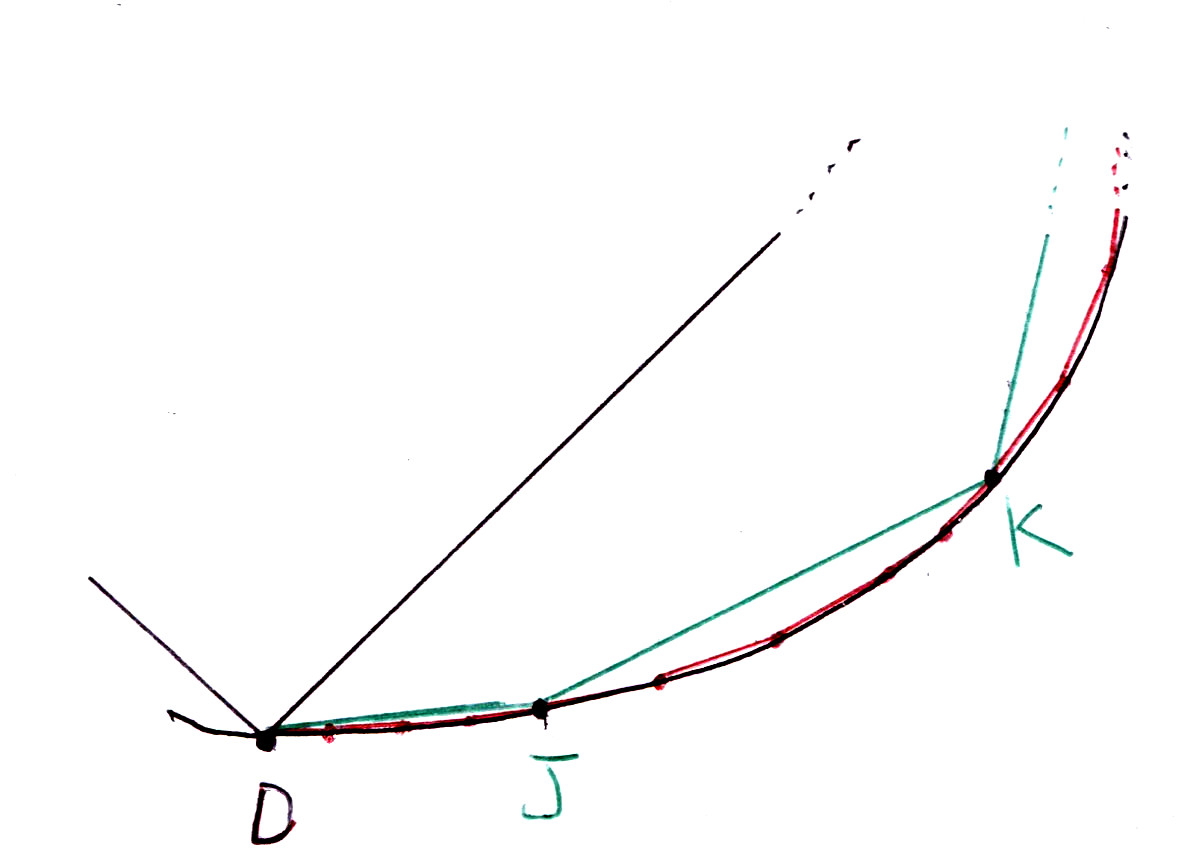
\includegraphics[width=0.5\textwidth]{image/pi_nombre/courbe4.jpg}
		
		\caption{Lignes brisées qui suivent une subdivision de plus en plus fine de la courbe comprise entre $A$ et $B$. La dernière figure représente un zoom sur celle de droite, là où on a mis une accolade.} \label{fig_ligne_brisee}
	\end{figure}

	Il faut aussi que les points de la ligne brisée soient ordonnés sur la courbe (on veut éviter les allers-retours, voir figure \ref{fig_aller_retour}). Cela fait appel à des axiomes d'ordonnancements de points le long d'un chemin. Cela se fait de la manière suivante\,: on définit une relation ternaire entre trois points : on écrira $A\star B\star C$ pour signifier que $B$ est entre $A$ et $C$ le long de la courbe. Cela peut se faire de manière axiomatique. Nous le ferons dans le chapitre \ref{chap_angle} pour les points alignés sur une droite. L'axiomatisation sur une courbe est similaire. L'extension de ces axiomes sur une courbe ne pose pas de problème en principe.

	\begin{figure}
		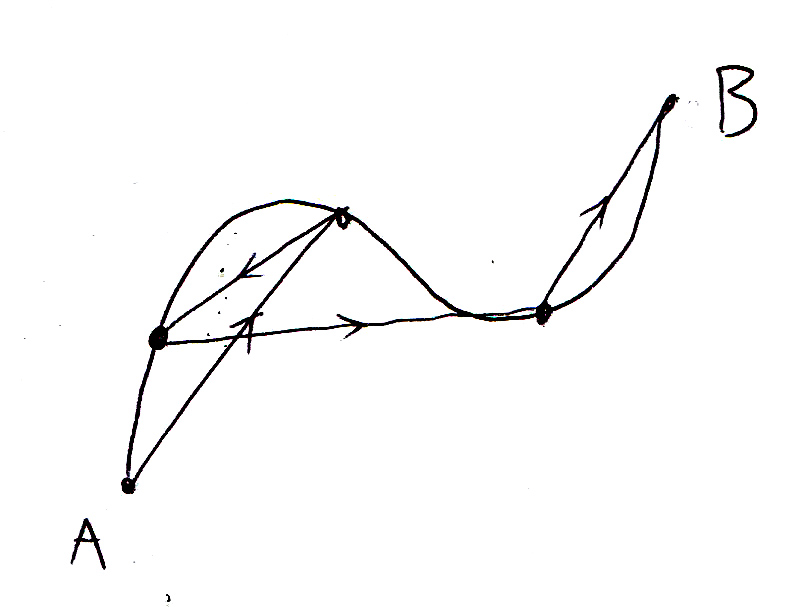
\includegraphics[width=0.4\textwidth]{image/pi_nombre/aller_retour2.jpg}
        \hfill 
        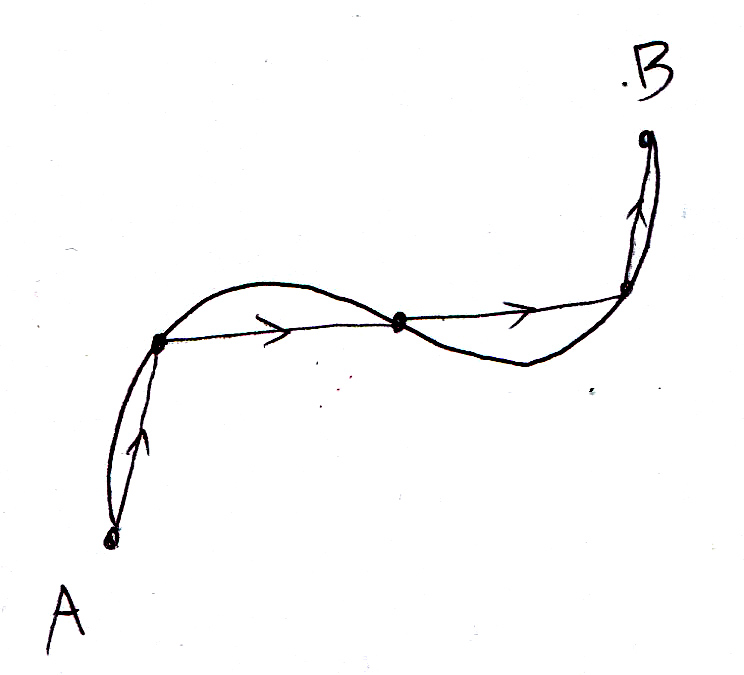
\includegraphics[width=0.4\textwidth]{image/pi_nombre/aller_retour1.jpg}
		\caption{À gauche\,: la ligne brisée fait un aller-retour. À droite\,: la ligne brisée ne fait pas d'aller-retour.}
		\label{fig_aller_retour}
	\end{figure}


	Les conditions de validité d'une telle définition ne sont pas si évidentes. D'abord, il faut s'assurer qu'il est bien possible de passer à la limite d'une subdivision infinie et qu'il est toujours possible de calculer la somme des mesures de chaque petit segment. Il existe des contres-exemples, par exemple des courbes qui occupent une aire finie mais dont le périmètre est infini\,; cela pose des problèmes dans le calcul (j'en mets un connu en annexe \ref{app_flocon}). Pour éviter les cas pathologiques, on se contentera de définir la longueur sous réserve d'existence de la limite de la longueur des lignes brisées (s'il est impossible de calculer cette limite, on décrètera que la longueur de la courbe n'est pas définie). 

	Ensuite, il faut s'assurer que lorsque l'on affine la subdivision, elle remplit bien toute la courbe\,: en effet, on pourrait ajouter une infinité de points mais seulement sur la première moitié de la courbe, et ainsi la longueur serait sous-estimée (voir figure \ref{fig_defaut_longueur}). 

	\begin{figure}
		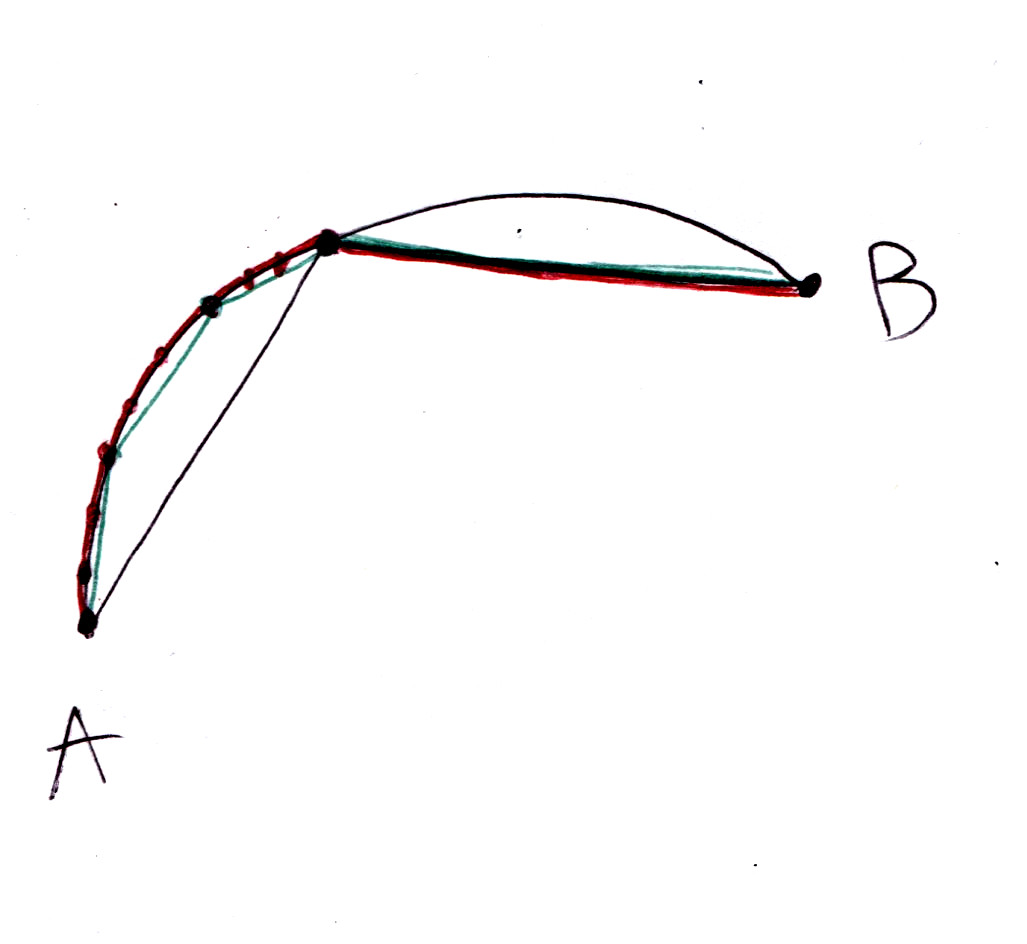
\includegraphics[width=0.4\textwidth]{image/pi_nombre/defaut_longueur.jpg}
		\caption{On approche la longueur de la courbe comprise entre $A$ et $B$ par des lignes brisées de plus en plus fines, mais on oublie de raffiner la subdivision sur toute une partie de la courbe. Ainsi, même la  mesure de la ligne brisée rouge est une mauvaise approximation de la longueur de la courbe.}\label{fig_defaut_longueur}
	\end{figure}

	Pour résoudre ce problème, on demande que la série de subdivisions de la courbe soit dense. Cela signifie que si l'on choisit un point arbitraire $M$ sur la courbe, et un rayon $r$ (strictement positif) arbitrairement petit, alors notre série de subdivision parviendra toujours à envoyer au moins un point dans la sphère de centre $M$ et de rayon $r$ (Voir figure \ref{fig_densite}). 

	\begin{figure}
		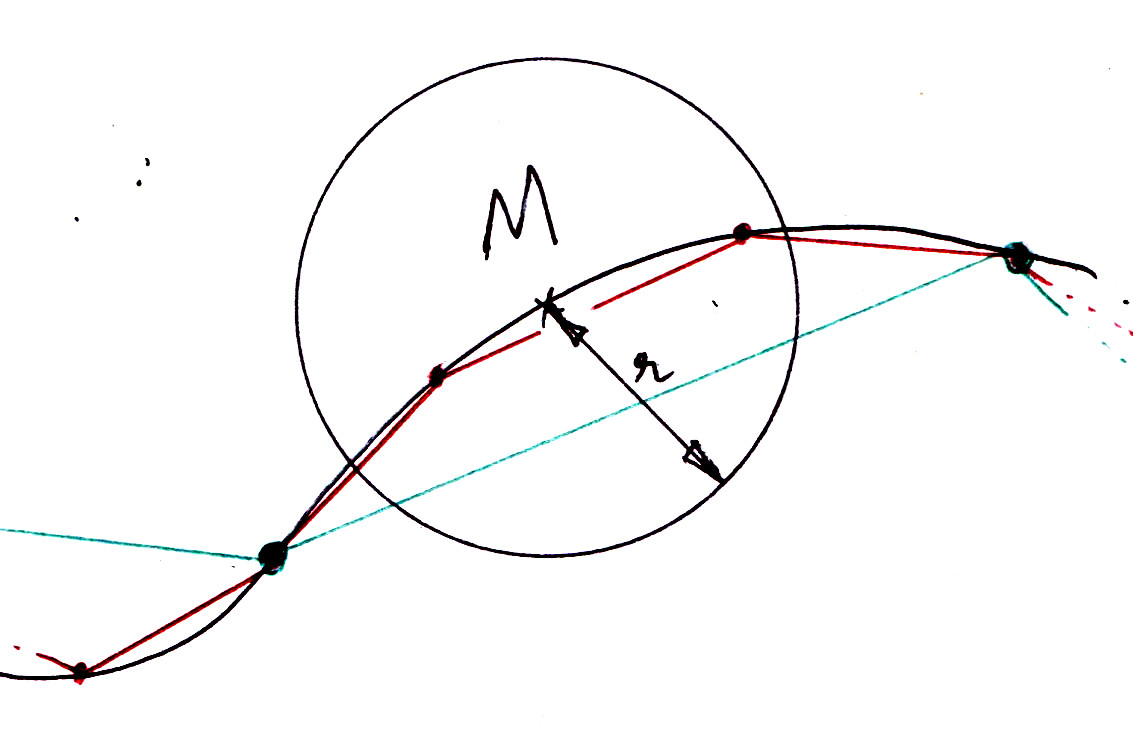
\includegraphics[width=0.5\textwidth]{image/pi_nombre/densite.jpg}
		\caption{Illustration du concept de densité. Ici, la subdivision en ligne brisée verte ne satisfait pas la condition requise, alors que la rouge oui.}\label{fig_densite}
	\end{figure}

	J'attire votre attention sur le caractère arbitrairement petit du nombre $r$. Cela signifie que si l'on prend n'importe quel point de la courbe, on pourra toujours trouver une subdivision assez fine pour qu'elle ait au moins un point aussi proche que l'on veut du point $M$. Cette propriété de densité assure que lorsque le nombre de points de la ligne brisée tend vers l'infin (ou que le rayon de la boule tend vers zéro), toute la courbe est remplie par la subdivision de la ligne brisée. Et histoire d'être sûr, il faudrait assurer que tous les points de la subdivision précédente sont contenus dans la subdivision suivante. C'est une manière de \og{}raffiner\fg\, la subdivision.

\section{Périmètre d'un cercle}

	Il est temps de commencer à approcher la longueur d'un cercle. Pour commencer nous allons considérer un cercle de rayon $R=1$. Nous allons appeler $P$ son périmètre. C'est le nombre que l'on se propose de calculer. La méthode d'Archimède a consisté à donner des encadrements de plus en plus fins de ce périmètre en encadrant géométriquement le cercle par des polygones réguliers inscrits et en inscrivant le cercle dans des polygones réguliers. Considérons une première étape constituée par une inscription d'hexagones réguliers.
	\begin{figure}
		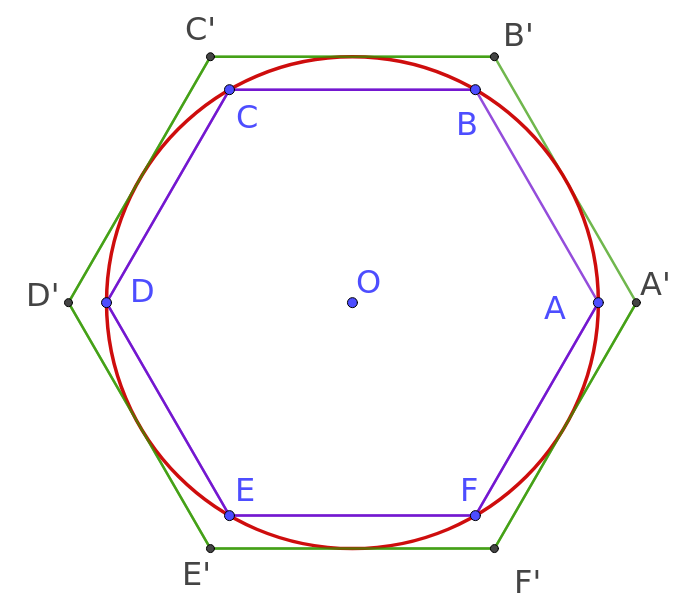
\includegraphics[width=0.5\textwidth]{image/pi_nombre/poly_inscrit.png}
		\caption{Hexagones réguliers. Le bleu est inscrit dans le cercle (chaque sommet appartient au cercle). Le vert est circonscrit au cercle (des parties du cercle touchent les côtés de cet hexagone). L'hexagone vert a ses côtés parallèles au bleu.}
	\end{figure}

	Calculons les périmètres de ces deux hexagones. Tout d'abord, on sait que $OA=1$ puisque c'est un rayon du cercle. Ensuite, joignons les sommets opposés de l'hexagone régulier. Cela forme 6 triangles isocèles dont les côtés égaux mesurent 1. Cependant, vu que l'on a partitionné un tour complet en six secteurs d'angles de mesures égales, alors chaque angle au centre mesure 360°/6=60°. Mais comme la somme des angles d'un triangle vaut 180° et que les deux autres angles sont égaux, on trouve facilement que les trois angles de chaque triangle mesurent tous 60°. Nous avons donc affaire à six triangles équilatéraux. On voulait calculer le périmètre de l'hexagone, mais en fait, chacun de ses côtés mesure le rayon du cercle, et donc, le périmètre mesure $6\times OA=6$. Ainsi, on sait que le périmètre du cercle est légèrement plus grand que 6.

	De même, on comprend facilement que le périmètre du grand hexagone mesure $6\times OA'$. Mais il nous faut calculer $OA'$.
	Considérons le triangle $OA'B'$. Traçons la médiatrice du segment $[A'B']$. Elle coupe $[A'B']$ perpendiculairement en son milieu, en $M$ et passe par $O$. Elle constitue un axe de symétrie du triangle considéré. De plus, $[OM]$ est un rayon du cercle, donc $OM=1$. Le triangle $OMA'$ est rectangle en $M$, donc d'après le théorème de Pythagore, on a
	\begin{equation}
		OA'^2=OM^2+MA'^2. \nonumber
	\end{equation}
	Mais $OM=1$ et puisque $OA'=A'B'$ et que $M$ est le milieu de $A'B'$, $MA'=\frac{OA'}{2}$. Ainsi, l'égalité de Pythagore devient
	\begin{equation}
		OA'^2=1^2+\(\frac{OA'}{2}\)^2 = 1+\frac{OA'^2}{2^2}=1+\frac{OA'^2}{4} \nonumber
	\end{equation}
	Si l'on regroupe les termes contenant $OA'$ à gauche de l'équation, on obtient
	\begin{equation}
		OA'^2+\frac{1}{4}OA'^2=1 \Leftrightarrow \(1-\frac{1}{4}\)OA'^2=1 \Leftrightarrow \frac{3}{4}OA'^2=1 \Leftrightarrow OA'^2=\frac{4}{3}.\nonumber
	\end{equation}
	On en déduit que
	\begin{equation}
		OA'=\sqrt{\frac{4}{3}}=\frac{\sqrt{4}}{\sqrt{3}}=\frac{2}{\sqrt{3}}. \nonumber
	\end{equation}
	Et enfin, le périmètre du grand hexagone mesure $6\times OA'=12/\sqrt{3}\approx6,93$.

	On obtient donc une première approximation de $\pi$\,:
	\begin{equation}
		6<2\pi<9.93 \quad\text{et donc}\quad 3<\pi<4.965\nonumber
	\end{equation}

	Cette approximation est très grossière. Que faire\,? Inspirés par la définition des longueurs des courbes dans la section précédente, divisons notre subdivision en deux, autrement dit, multiplions par deux le nombre de côtés de l'hexagone inscrit. Nous obtenons la figure \ref{fig_doubler_hex}.

	\begin{figure}
		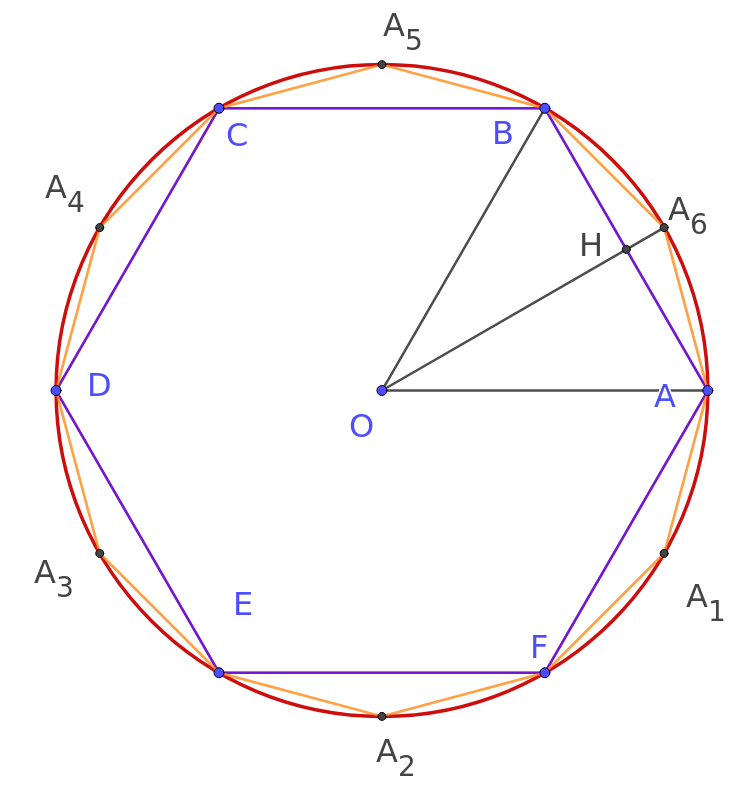
\includegraphics[width=0.6\textwidth]{image/pi_nombre/doubler_hex.png}
		\caption{Doublement du nombre de côté de l'hexagone.}\label{fig_doubler_hex}
	\end{figure}

	\noindent 3) On appelle $c_1$ la mesure du côté du dodécagone inscrit et $L_1$ son périmètre, et $d_1$ la mesure du côté du dodécagone circonscrit, et $P_1$ son périmètre. Calculer tous ces nombres. En déduire un encadrement plus fin de $\pi$.

	Supposons avoir subdivisé $n$ fois l'hexagone de départ. On aurait alors multiplié le nombre de côté par 2, $n$ fois, à savoir, par $2\times2\times2\times\ldots\times 2$ où 2 apparaît $n$ fois. Il existe une notation économique pour noter ce nombre\,: $2^n$. Au rang $n$, notons $c_n$ la mesure d'un côté de ce polygone, et notons $L_n$ la longueur de ce polygone. Puisqu'au rang $n$ il y a $6\times 2^n$ côtés, nous avons\,: $L_n=6\times 2^n c_n$. De plus, nous savons qu'au rang zéro, $c_0=1$, nous l'avons calculé plus haut.
	Pour automatiser la procédure, nous voudrions voir comment varie $c_n$ lorsque l'on passe de $n$ à $n+1$. Ensuite, un programme numérique poura aisément itérer le processus autant de fois que le permettent les ressources informatiques, étant donné le point de départ.

	Regardons comment cela se passe sur la figure \ref{fig_iter}. Supposons que le segment $[AB]$ représente le côté de longueur $c_n$. Lorsque l'on double le nombre de côtés, on construit le point $E$ à l'intermédiaire, et ainsi, $AE=EB=c_{n+1}$. Ainsi, $(OE)$ est la médiatrice du segment $[AB]$. 
	\begin{figure}
		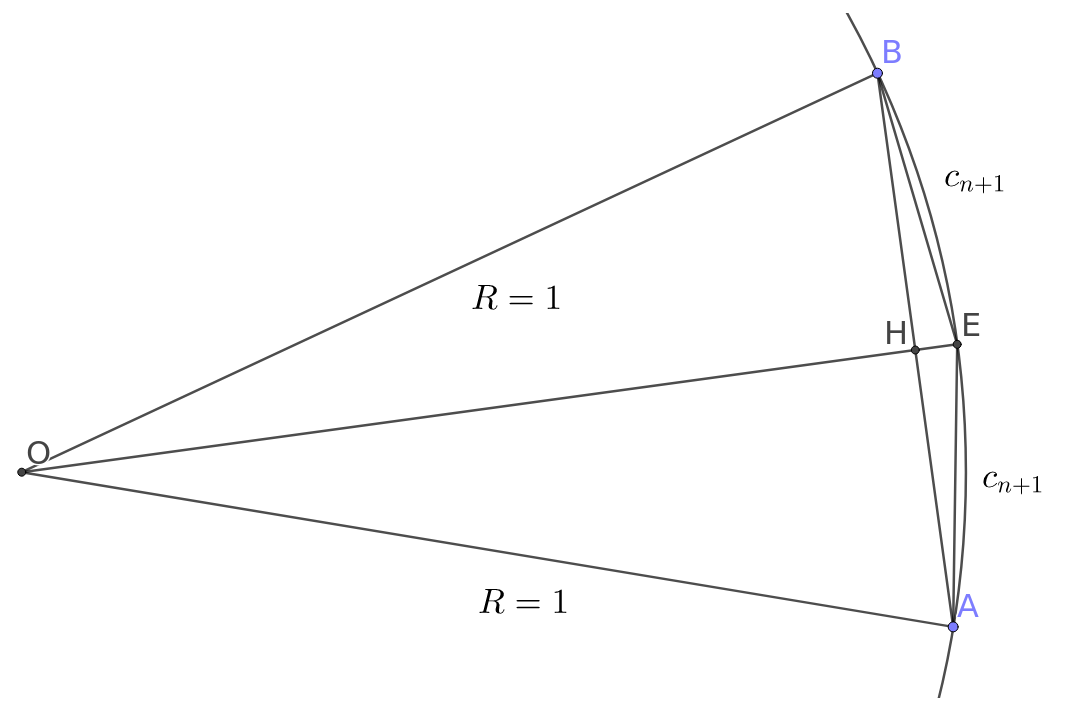
\includegraphics[width=0.6\textwidth]{image/pi_nombre/iteration.png}
		\caption{Itération pour passer du calcul de $c_n$ à celui de $c_{n+1}$.}\label{fig_iter}
	\end{figure}

	Nommons $H$ l'intersection de $(AB)$ et de $(OE)$, qui sont perpendiculaires. Dans le triangle $OAH$ rectangle en $H$, le théorème de Pythagore nous donne $OA^2=AH^2+OH^2$. Mais $OA=1$ et $AH=AB/2=c_n/2$. Après quelques manipulations, on obtient 
	\begin{equation}
		OH=\sqrt{1-\(\frac{c_n}{2}\)^2}=\sqrt{1-\frac{c_n^2}{4}}. \nonumber
	\end{equation}
	De là, on tire $HE=1-OH=1-\sqrt{1-\frac{c_n^2}{4}}$. Et enfin, dans le triangle $AHE$ rectangle en $H$,
	\begin{equation}
		c_{n+1}=AE=\sqrt{AH^2+HE^2}=\sqrt{\(\frac{c_n}{2}\)^2+\(1-\sqrt{1-\frac{c_n^2}{4}}\)^2}.\nonumber
	\end{equation}
	En développant l'identité remarquable et en simplifiant, on trouve enfin
	\begin{equation}
		c_{n+1}=\sqrt{2}\sqrt{1-\sqrt{1-\frac{c_n^2}{4}}} \label{eq_cnpu}
	\end{equation}
	Et là, on a gagné. En effet, on connaît la valeur de $c_0$ (cela mesure 1) et on sait comment passer de $c_n$ à $c_n+1$. D'ailleurs, remarquons que l'on retrouve bien le passage de $c_0$ à $c_1$ que l'on a fait un peu plus haut\,:
	\begin{equation}
		c_1=\sqrt{2}\sqrt{1-\sqrt{1-\frac{c_0^2}{4}}} = \sqrt{2-2\sqrt{1-\frac{1}{4}}}=\sqrt{2-\sqrt{3}}.\nonumber
	\end{equation}

	\usemintedstyle{bw}

	Dans un simple tableur, voici comment il suffirait de procéder pour approcher la valeur de $\pi$ (voir figure \ref{fig_approx_pi}).
	Dans la colonne $A$, on représente le nombre d'itérations $n$. Dans la colonne $B$, on représente le nombre $2^n$. Pour ce faire, il suffit d'écrire la formule \mintinline{python}{=2^A2} dans la case B2, puis d'étendre la formule sur toute la colonne. Cela donne un ordre de grandeur du nombre de côtés. Ensuite, il faut s'occuper de la colonne des côtés. On commence par itérer la valeur 1 dans la case $C2$. Ensuite, dans la case $C3$, on rentre la formule suivante\,: \mintinline{python}{=RACINE(2)*RACINE(1-RACINE(1-C2*C2/4))}. Puis on étend. Enfin, on s'occupe de la colonne des longueurs. Dans la colonne des longueurs, on rentre simplement, en case $D2$, la formule \mintinline{python}{=6*B2*C2}. Puis on étend. Et pour obtenir une approximation du nombre $\pi$, on divise par deux (dernière colonne).
	\begin{figure}
		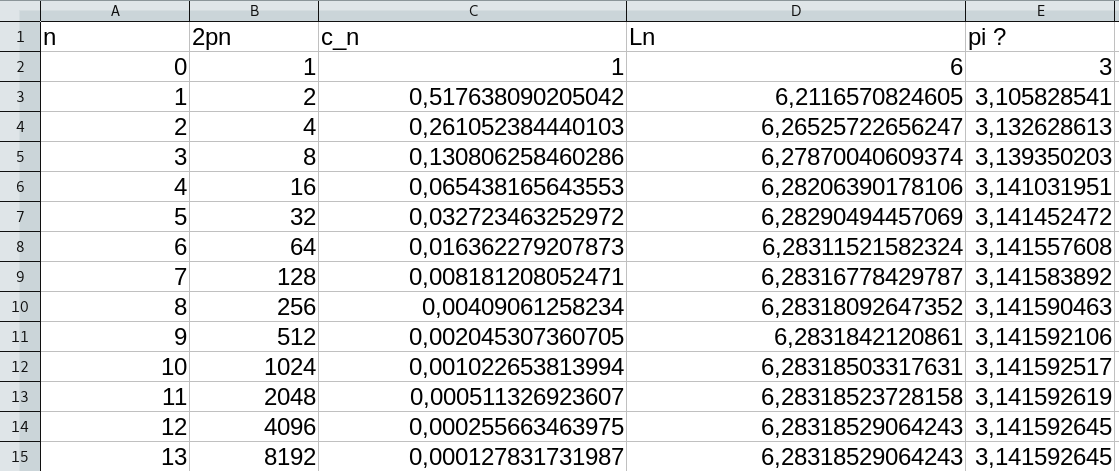
\includegraphics[width=\textwidth]{image/pi_nombre/approx_pi.png}
		\caption{Approximation de $\pi$ avec un tableur.}\label{fig_approx_pi}
	\end{figure}


	Pour être véritablement complet, il faudrait aussi faire de même avec le polygone circonscrit au cercle. Nous laissons cela en exercice au lecteur\,!

	\paragraph{Exercice} On considère l'hexagone circonscrit au cercle de rayon 1. De même, on va multiplier par deux le nombre de ses côtés de telle sorte que chaque côté soit tangent au cercle, et qu'à chaque itération, le polygone est régulier. Démontrer que si l'on note $d_n$ la mesure du côté du polygone circonscrit au cercle, et $P_n$ son périmètre, alors on a
	\begin{align}
		d_0&=\frac{2}{\sqrt{3}} \\
		P_0&=\frac{12}{\sqrt{3}} \\
		d_{n+1}&=\sqrt{2}\sqrt{\sqrt{\frac{d_n^2}{4}+1}-1} \label{eq_dnpu}\\
		P_n&=6\times 2^n d_n.
	\end{align}

\section{Conclusion\,: $\pi$ est-il vraiment un nombre\,?}
	Il nous reste une dernière chose à démontrer\,: que le nombre $\pi$ ainsi calculé ne dépend pas du rayon du cercle. En effet, jusqu'ici nous n'avons calculé que le périmètre d'un cercle de rayon 1, et nous avons divisé par son diamètre particulier ($D=2R=2$) pour obtenir une approximation de $\pi$. Qu'obtiendrions-nous si nous faisons le même processus sur n'importe quel cercle\,?

	C'est le théorème de Thalès qui nous permet de vérifier que le nombre $\pi$ est invariant par modification du cercle.

	\begin{figure}
		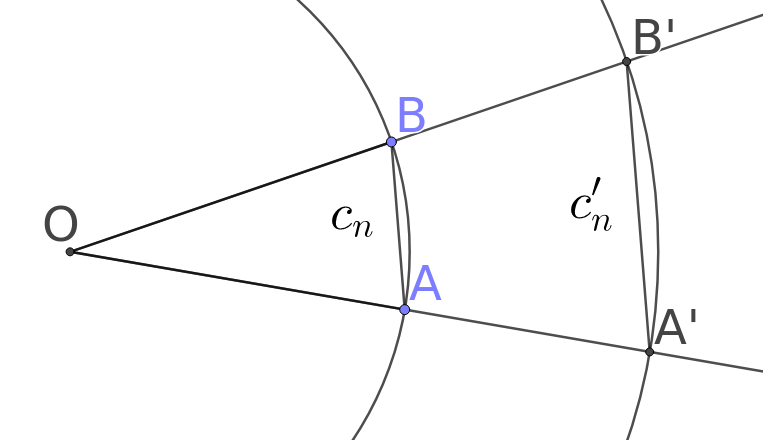
\includegraphics[width=0.6\textwidth]{image/pi_nombre/thales.png}
		\caption{Illustration d'une étape du calcul du périmètre des deux cercles emboîtés.}\label{fig_semblabilite}
	\end{figure}


	Considérons deux cercles de rayons différents et procédons de même pour approcher leur périmètre\,: on subdivise les cercles en des polygones réguliers inscrits. Déplaçons les figures de telle sorte que les deux centres des deux cercles coïncident, et qu'à l'étape $n$, les demi-droites formées par les centres des cercles et les sommets des polygones coïncident. C'est toujours possible, car au rang $n$, l'angle formé par les deux sommets les plus proches du polygone et le centre sont identiques (on divise un tour complet en $6\times 2^n$ secteurs d'angles égaux de même mesure). Nommons $c_n$ le côté du polygone inscrit du petit cercle, et $c_n'$ le côté du polygone inscrit du grand cercle (voir figure \ref{fig_semblabilite}). Les deux triangles $OAB$ et $OA'B'$ sont semblables. En effet, ils sont isocèles, et partagent un angle (au centre du cercle). Ainsi, $\widehat{OAB}=\widehat{OA'B'}=\widehat{OBA}=\widehat{OB'A'}$. Par propriété des angles alternes-internes, $(AB)\sslash(A'B')$. On peut donc utiliser le théorème de Thalès\,:
	\begin{equation}
		\frac{OA}{OA'}=\frac{AB}{A'B'}. \nonumber	
	\end{equation}
	En notant $R=OA$ et $R'=OA'$, on obtient alors
	\begin{equation}
		\frac{R}{R'}=\frac{c_n}{c_n'}\quad\text{donc}\quad \frac{c_n}{R}=\frac{c_n'}{R'}. \nonumber
	\end{equation}
	Au rang zéro, le périmètre de l'hexagone du petit cercle mesure $L_0=6R$ et celui du grand, $L_0'=6R'$. Au rang $n$, on a tout simplement $L_n=6\times 2^n c_n $ et $L_n'=6\times 2^n c_n' $.
	La valeur approchée au rang $n$ de $\pi$ pour le petit cercle vaut donc\,:
	\begin{equation}
		\pi_n=\frac{1}{2R}6\times 2^n c_n = 3\times 2^n \frac{c_n}{R}.\nonumber
	\end{equation}
	Mais comme $c_n/R=c_n'/R'$, en fait, $\pi_n=\pi_n'$. 

	On vient de démontrer que le calcul de $\pi$ ne dépend pas de la taille du cercle considéré, et donc, on peut raisonnablement poser\,:
	\begin{equation}
		\pi=\lim\limits_{n\to\infty}\pi_n \nonumber
	\end{equation}

	{\bfseries Et donc $\pi$ est bien un nombre. CQFD\,!!!}

	Remarque : il reste une arnaque dans la démonstration. À aucun moment nous n'avons démontré que les suites de nombres $(L_n)$ et $(P_n)$ convergeaient bien vers un nombre, et encore moins que c'était le même nombre. Un constat empirique ne vaut pas une démonstration mathématique. Nous la reportons en annexe \ref{app_conv}. 

\section{Flash forward\,: calculer $\pi$ à l'aide des fonctions trigonométriques}

	Considérons un cercle trigonométrique dans lequel on inscrit un polygone régulier à $n$ sommets. Alors l'angle au centre formé par deux sommets consécutifs mesure $2\pi/n$. Un simple calcul de trigonométrie permet de vérifier que la distance qui sépare deux sommets consécutifs mesure $2\sin(\pi/n)$. Le périmètre d'un tel polygone mesure alors $P_n=2n\sin(\pi/n)$ et donc on peut prouver que
	\begin{equation}
		\pi=\lim\limits_{n\to\infty}n\sin\(\frac{\pi}{n}\).\label{eq_serpent}
	\end{equation}
	Mais à ce stade, c'est un peu le serpent qui se mord la queue...


\newpage
    